\section{Aufbau}
\label{sec:Aufbau}

\begin{figure}
\centering
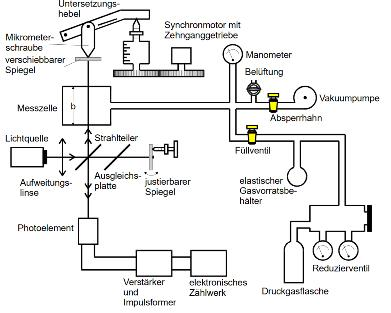
\includegraphics[scale=0.5]{content/images/aufbau.jpg}
\caption{Schematischer Aufbau eines Michelson-Interferometers\cite{V401}}
\label{fig:Aufbau}
\end{figure}

\noindent Der Versuch wird gemäß Abbildung \ref{fig:Aufbau} aufgebaut. Der justierbare Spiegel wird so ausgerichtet, das die am Detektor auftreffenden Strahlen des justierbaren und des verschiebbaren Spiegels
am selben Punkt auftreffen. Anschließend wird eine Zerstreuungslinse in den Strahlengang eingebracht, sodass Interferenzmuster entstehen. Der in Strahlrichtung verschiebbare Spiegel wird über einen Motor bewegt, sodass die Interferenzringe sich über das Photoelement bewegen. Dies registriert die Lichtintensitätsschwankungen und wandelt sie in elektrische Impulse um, die über einen Verstärker von einem Zählwerk erfasst werden.
Mit der Vakuumpumpe kann die Luft aus der Messzelle entfernt und über ein Ventil wieder eingelassen werden. In diesem Versuch wird nur der Brechungsindex in Luft untersucht, sodass keine Gasbehälter benötigt werden.